\documentclass[11pt]{amsart}
\pdfoutput=1
\usepackage{amsmath, amssymb, amsthm, graphicx, subfig, mathrsfs, calc, xspace,
  mathtools, ifthen, booktabs, longtable, comment, setspace, verbatim,
  placeins, abraces}
\usepackage[colorlinks=true]{hyperref}
\hypersetup{urlcolor=blue, citecolor=red}
\newlength{\figWidthA}
\newlength{\figWidthB}

% General
\newcommand{\xth}[1][th]{\textsuperscript{#1}\xspace}
\newcommand{\set}[2]{\ifthenelse{\equal{#2}{}}{\{#1\}}{\{#1 \mid #2\}}}
\newcommand{\ol}{\overline}
\newcommand{\s}{\sigma}
\newcommand{\nats}{\mathbb{N}}
\newcommand{\ints}{\mathbb{Z}}
\newcommand{\G}{\mathscr{G}}
\newcommand{\V}[1][G]{V(#1)}
\newcommand{\E}[1][G]{E(#1)}
\newcommand{\N}[2][]{\ifthenelse{\equal{#1}{}}{N(#2)}{N_{#1}(#2)}}
\renewcommand{\deg}[2][]{\ifthenelse{\equal{#1}{}}{d(#2)}{d_{#1}(#2)}}
\newcommand{\size}[1]{\##1}

\newcommand{\gamename}[1]{\ifthenelse{\equal{\showinggamename}{false}}%
  {}{^{#1}}}
\newcommand{\showgame}{\def\showinggamename{true}}
\newcommand{\hidegame}{\def\showinggamename{false}}
\newcommand{\showhere}[1]{\showgame#1\hidegame}
\hidegame

% Parallel chip-firing
\newcommand{\pos}[2][\s]{#1_{#2}}
\newcommand{\chips}[3][\s]{#1_{#3}(#2)}
\newcommand{\receiving}[3][\s]{\Phi\gamename{#1}_{#3}(#2)}
\newcommand{\firing}[3][\s]{F\gamename{#1}_{#3}(#2)}
\newcommand{\pfp}[2][\s]{F\gamename{#1}(#2)}
\newcommand{\period}[1][\s]{T\gamename{#1}}
\newcommand{\pfpverts}[2][\s]{\tau\gamename{#1}(#2)}
\newcommand{\pfpedges}[3][\s]{\pi\gamename{#1}(#2,#3)}
\newcommand{\misb}[4][\s]{m\gamename{#1}_{#2}(#3,#4)}
\newcommand{\sctr}[1]{\mathcal{X}(#1)}
\newcommand{\mots}[1][\s]{M\gamename{#1}}
\newcommand{\pfps}[1][\s]{P\gamename{#1}}
\newcommand{\cpfps}[1][\s]{Q\gamename{#1}}

% Theorem
\newtheorem{thm}{Theorem}[section]
\newtheorem{lem}[thm]{Lemma}
\newtheorem{cor}[thm]{Corollary}
\newtheorem{conj}[thm]{Conjecture}
\numberwithin{equation}{section}

\begin{document}

\setlength\figWidthA{.72\textwidth}
\setlength\figWidthB{.28\textwidth}

\title[Motors and Impossible Firing Patterns in the PCFG]{Motors and Impossible
  Firing Patterns in the\\Parallel Chip-Firing Game}
\author{Tian-Yi Jiang, Ziv Scully, Yan X Zhang}
\address{Massachusetts Institute of Technology}
\email{jiangty@mit.edu, ziv@mit.edu, yanzhang@post.harvard.edu}
\begin{abstract}
The \emph{parallel chip-firing game} is an automaton on graphs in which
vertices ``fire'' chips to their neighbors. This simple model contains much
emergent complexity and has many connections to different areas of
mathematics. In this work, we study \emph{firing sequences}, which describe
each vertex's interaction with its neighbors in this game. First, we introduce
the concepts of \emph{motors} and \emph{motorized games}. Motors both
generalize the game and allow us to isolate local behavior of the (ordinary)
game. We study the effects of motors connected to a tree, and show that
motorized games can be transformed into ordinary games if the motor's firing
sequence occurs in some ordinary game. Then, we completely characterize the
periodic firing sequences that can occur in an ordinary game, which have a
surprisingly simple combinatorial description.

\end{abstract}
\maketitle

\section{Introduction}

\subsection*{Background}
The \emph{parallel chip-firing game}, also known as the \emph{discrete
  fixed-energy sandpile model}, is an automaton on graphs in which vertices
that have at least as many chips as incident edges ``fire'' chips to their
neighbors. In graph theory, it has been studied in relation with the critical group of graphs~\cite{biggs}. In computer science, it is able to simulate any
two-register machine and is thus universal~\cite{universality}. As a specific case of the \emph{abelian sandpile model}, which is itself a generalization of a sandpile model introduced by Bak, Tang, and Weisenfeld~\cite{BTWcriticality, BTWmoreCriticality} in the study of self-organized criticality, it has even more links with other fields.

\subsection*{The Game}
The parallel chip-firing game is played on a graph as follows:
\begin{itemize}
\item At first, a nonnegative integer number of chips is placed on each vertex
  of the graph.
\item The game then proceeds in discrete turns. Each turn, a vertex checks to
  see if it has at least as many chips as incident edges.
\begin{itemize}
\item If so, that vertex \emph{fires}.
\item Otherwise, that vertex \emph{waits}.
\end{itemize}
\item To fire, a vertex passes one chip along each of its edges. All vertices
  that fire in a particular turn do so in parallel.
\item Immediately after firing or waiting, every vertex receives any chips that
  were fired to it.
\end{itemize}
Here we will only consider games on finite, undirected, connected graphs,
though the definition of the game can be easily generalized for arbitrary
multidigraphs. An example game is illustrated in Figure~\ref{example}. Given a
parallel chip-firing game as $\s$, we represent the chip configuration at a
particular time $t \in \nats$ as $\pos{t}$.
\begin{figure}[h]
\centering
\subfloat{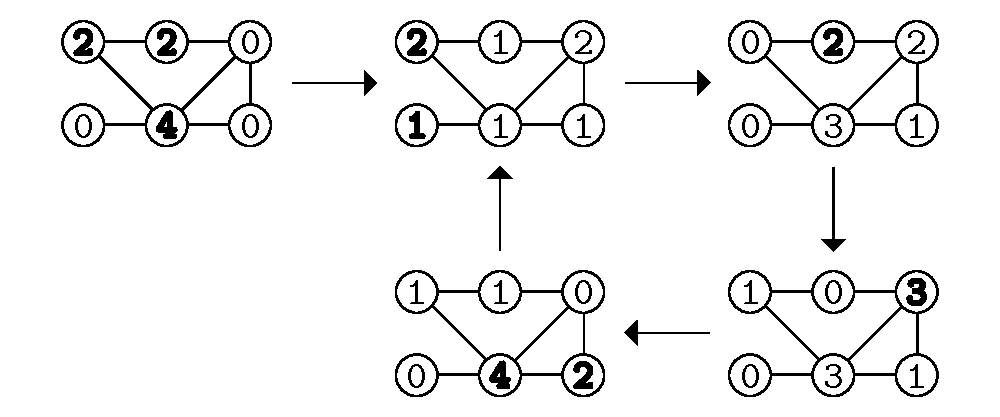
\includegraphics[width=\figWidthA]{Figures/example}}
\subfloat{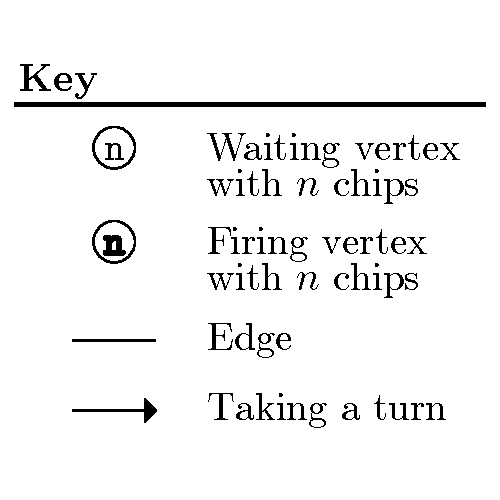
\includegraphics[width=\figWidthB]{Figures/keyShort}}
\caption{A parallel chip-firing game. From an initial position in the upper
  left, the game eventually enters a period of length 4.}
\label{example}
\end{figure}

The total number of chips on all vertices of the graph is constant throughout a
game, so there are finitely many possible positions in every game. Therefore,
every game eventually reaches a position $\pos{t}$ that is identical to a later
position $\pos{t+p}$ for some $t,p \in \nats$ with $p > 0$. (We write $\pos{t}
= \pos{t+p}$.) The game is deterministic, so $\pos{t+n} = \pos{t+n+p}$ for all
$n \in \nats$. Thus, every parallel chip-firing game is eventually periodic.

In this paper, we concern ourselves with both \emph{firing sequences} and
\emph{periodic firing patterns} of vertices. Each is a binary string
representing whether or not a particular vertex fires or waits each turn. The
sequence covers all times from 0 to infinity, while the periodic pattern covers
just one period.

\subsection*{Previous Work}
The periodicity of the parallel chip-firing game gives rise to two
questions. First, what characteristics of a game and its underlying graph
determine the length of a period? It is known exactly what periods are possible
on certain classes of graphs, such as trees~\cite{bitarGoles}, simple
cycles~\cite{cycle}, the complete graph~\cite{levine}, and the complete
bipartite graph~\cite{jiang}. Kiwi et al.~\cite{kiwiEtAl} constructed graphs on
which the period of games can grow exponentially with polynomial increase in
the number of vertices. There are also results regarding the total number of
chips in a game. Kominers and Kominers~\cite{kominers} showed that games with a
sufficiently large density of chips must have period~1. Dall'Asta~\cite{cycle}
and Levine~\cite{levine}, in their respective characterizations of periods on
cycles and complete graphs, related the total number of chips to a game's
\emph{activity}, the fraction of turns during which a vertex fires. The
denominator of the activitymust divide the period.

Second, we notice that some but not all positions $\pos{t}$ are
\emph{periodic}, satisfying $\pos{t} = \pos{t+p}$ for some positive $p \in
\nats$. What characterizes periodic positions? This problem has not been as
extensively studied. Dall'Asta~\cite{cycle} characterized the periodic
positions of games on cycles.

\subsection*{Our Results}
We hope to advance the understanding of both of these questions through the
study of firing sequences and periodic firing patterns.

After precisely defining the parallel chip-firing game in Section~\ref{pres},
the first half of the paper develops a new tool for studying the chip-firing
game: \emph{motors}, vertices that fire with a regular pattern independent of
normal chip-firing rules. Games with motors are called \emph{motorized
  games}. Motors allow us to study the behavior of subgraphs in ordinary
parallel chip-firing games. In Section~\ref{motors} we show that vertices
always ``follow'' a motor in periodic motorized games on trees. In
Section~\ref{simulatingMotors}, we prove that periodic motorized games can be
transformed into ordinary games as long as the firing sequence of each motor
occurs in an ordinary game.

The second half of the paper characterizes the possible periodic firing
patterns in parallel chip-firing games. Section~\ref{binSeq} briefly steps away
from the game to study certain signed sums of periodic binary sequences. The
result is an inequality applicable to edges of the graph of a parallel
chip-firing game. In Section~\ref{nonclumpiness}, we sum this inequality over
all relevant edges to show that periodic firing patterns with both consecutive
0s and consecutive 1s cannot occur in a parallel chip-firing game. This, along
with an already known construction, fully characterizes the periodic firing
patterns possible in parallel chip-firing games. Finally, in
Section~\ref{corollaries}, we examine some implications of this theorem.


\section{Preliminaries} \label{pres}

\subsection*{Definitions}
A \emph{parallel chip-firing game} $\s$ on a graph $G = (\V, \E)$ is a sequence
$(\pos{t})_{t \in \nats}$ of ordered tuples with natural number elements
indexed by $\V$. Each tuple represents the chip configuration at a particular
turn, where each element of the tuple is the number of chips on the
corresponding vertex. We define the following for all $v \in \V$:
\begin{align*}
  \N{v} &= \set{w \in \V}{\{v,w\} \in \E} \\
  \deg{v} &= \size{\N{v}} \\
  \chips{v}{t} &= \text{number of chips on $v$ in position $\pos{t}$} \\
  \firing{v}{t} &= \begin{cases}
    0 &\text{ if } \chips{v}{t} \leq \deg[]{v} - 1 \\
    1 &\text{ if } \chips{v}{t} \geq \deg[]{v}
  \end{cases} \\
  \receiving{v}{t} &= \sum_{\mathclap{w \in \N{v}}} \firing{w}{t}.
\end{align*}
In a parallel chip-firing game, $\pos{t}$ induces $\pos{t+1}$. For all $v \in
\V$,
\begin{equation}\label{gameDef}
  \chips{v}{t+1} = \chips{v}{t} + \receiving{v}{t} - \firing{v}{t}\deg[]{v},
\end{equation}
so an initial position suffices to define a game on a given graph. When
$\firing{v}{t} = 0$, we say $v$ \emph{waits} at $t$, and when $\firing{v}{t} =
1$, we say $v$ \emph{fires} at $t$.

A position $\pos{t}$ is \emph{periodic} if and only if there exists $p \in \nats$ such
that $\pos{t} = \pos{t+p}$. The minimum such $p$ for which this occurs is the
\emph{period} of $\s$ and is denoted $\period$. Abusing notation slightly, ``a
period'' of a game $\s$ may also refer to a set of times $\{t, t+1, \dots,
t+\period-1\}$, where $\pos{t}$ is periodic. The parallel chip-firing game is
deterministic and there are finitely many possible positions on a given graph
with a given number of chips, so for any game $\s$, there exists $t_0 \in
\nats$ such that $\pos{t}$ is periodic for all $t \geq t_0$. If the initial
position of a game is periodic, we may also call the game itself periodic.

\subsection*{Notation}
\newlength{\tablespace}
\setlength{\tablespace}{.3\baselineskip}
Definitions for invented notation are given in the section indicated in the
last column.\\

\showgame
\begin{centering}
  \begin{longtable}{l p{.65\textwidth} l}
    \toprule
    \multicolumn{2}{l}{\emph{Parallel Chip-Firing}} & \emph{Defined in} \\
    \midrule

    $\chips{v}{t}$ & Number of chips on vertex $v$ in position $\pos{t}$. &
    Section~\ref{pres} \vspace{\tablespace}\\

    $\pfp{v}$ & Periodic firing pattern of $v$. & Section~\ref{nonclumpiness}
    \vspace{\tablespace}\\

    $\firing{v}{t}$ & Indicates whether or not vertex $v$ fires in $\pos{t}$. &
    Section~\ref{pres} \vspace{\tablespace}\\

    $\receiving{v}{t}$ & Number of chips vertex $v$ will receive in $\pos{t}$.
    & Section~\ref{pres} \vspace{\tablespace}\\

    $\pat{v}{f}$ & Set of times for which a vertex $v$ waits (if $f = 0$) or
    fires (if $f = 1$) in $\s$. & Section~\ref{motors} \vspace{\tablespace}\\

    $\period$ & Period of $\s$. & Section~\ref{pres} \vspace{\tablespace}\\

    $\mots$ & Set of vertices that are motors in $\s$. & Section~\ref{motors}
    \vspace{\tablespace}\\

    $\pfps$ & Set of periodic firing patterns in $\s$. &
    Section~\ref{nonclumpiness} \vspace{\tablespace}\\

    $\cpfps$ & Set of clumpy periodic firing patterns in $\s$. &
    Section~\ref{nonclumpiness} \vspace{\tablespace}\\

    \toprule
    \multicolumn{3}{l}{\emph{Graphs}} \\
    \midrule

    $\V$ & \multicolumn{2}{l}{Vertex set of graph $G$} \vspace{\tablespace}\\

    $\E$ & \multicolumn{2}{l}{Edge set of graph $G$} \vspace{\tablespace}\\

    $\N[G]{v}$ & \multicolumn{2}{l}{Neighbors of vertex $v$.}
    \vspace{\tablespace}\\

    $\deg[G]{v}$ & \multicolumn{2}{p{.815\textwidth}}{The degree of vertex $v$
      in graph $G$.} \vspace{\tablespace}\\

    \toprule
    \multicolumn{3}{l}{\emph{Other}} \\
    \midrule

    $[a,b]$ & \multicolumn{2}{l}{The integer interval $\{a, a+1, \dots, b\}$.}
  \end{longtable}
\end{centering}
\hidegame

We leave out the subscript $G$ or superscript $\s$ if there is no ambiguity.


\section{Motors}\label{motors}

Let $G$ be a graph. Suppose we wish to study the periodic behavior of games on
$G$, focusing on a particular subgraph $H \subseteq G$. Consider
\begin{equation*}
  X = \set{v \in \V \setminus \V[H]}{\N{v} \cap \V[H] \neq \emptyset},
\end{equation*}
the set of vertices ``just outside'' of $H$. Knowing the initial chip
configuration on $\V[H] \cup X$ is in general not enough to determine all
subsequent configurations because vertices in $X$ may have interactions with
vertices outside of $\V[H] \cup X$. However, we do know that every vertex
assumes a pattern of firing and waiting that repeats periodically as soon as a
game reaches a periodic position. Therefore, we can simulate the presence of
the rest of $G$ by having each vertex in $X$ fire with a regular pattern
regardless of the number of chips it receives.

The $\emph{firing sequence}$ of a vertex $v$ in game $\s$ is the sequence
$(\firing{v}{t})_{t \in \nats}$. A \emph{motorized parallel chip-firing game},
or simply ``motorized game'', on $G$ is a game $\s$ obeying \eqref{gameDef}
with a non-empty set of \emph{motors} $\mots \subseteq \V$. Each motor follows
a predetermined firing sequence, firing without regard for the normal rules of
the parallel chip-firing game, which means, for example, that a motor may have
a negative number of chips. Put another way, for each $m \in \mots$,
$\firing{m}{t}$ does not depend on $\chips{m}{t}$. The term ``ordinary game''
refers to a game with no motors when there is ambiguity. A motorized game is
shown in Figure~\ref{motorizedTreeNoGlider}.

\begin{centering}
\begin{figure}[tbh]
  \subfloat{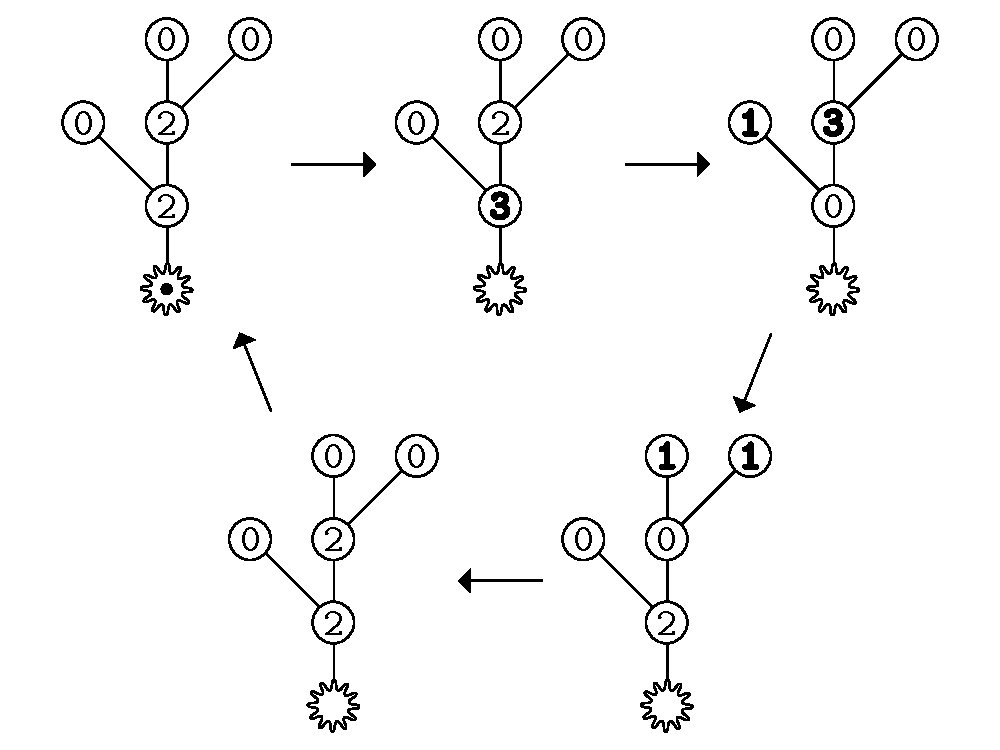
\includegraphics[width=\figWidthA]{Figures/motorizedTreeNoGlider}}
  \subfloat{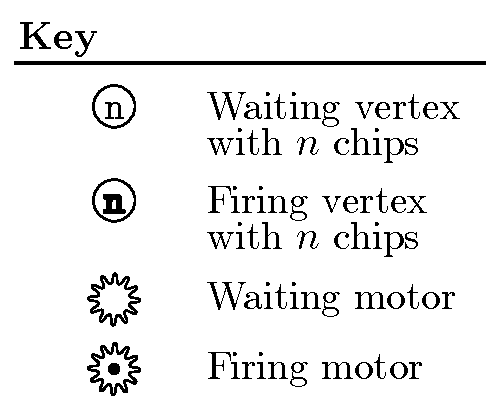
\includegraphics[width=\figWidthB]{Figures/keyShortish}}
  \caption{A motorized parallel chip-firing game. The motor has firing sequence
    $(1,0,0,0,0,1,0,0,0,0,\dots)$.}
  \label{motorizedTreeNoGlider}
\end{figure}
\end{centering}

If a motorized game $\s$ is eventually periodic (which is the case if every
motor's firing sequence is eventually periodic), then just as in an ordinary
game, every vertex fires the same number of times each period.  The proof is
identical to the proof of this fact for ordinary games~\cite{jiang}: all
neighbors of the vertex that fires the most times each period must also fire
that maximal number of times, and by induction, so do all vertices. (Recall
that we consider in this paper only connected graphs.)

We define
\[
  \pat{v}{f} = \set{t \in \nats}{\firing{v}{t} = f}.
\]
Call an interval $[a, b]$ with $a < b$ a \emph{max-clump} of $v \in \V$ if and
only if $[a, b] \subseteq \pat{v}{f}$ and $\firing{v}{a-1} = \firing{v}{b+1} =
1-f$, where $f \in \{0,1\}$. Given $v \in \V$, we can express $\nats$ as the
union of max-clumps of $v$ and times during which $v$ alternates between firing
and waiting.

The proof of Theorem~\ref{cheapLunch} follows the same structure as the proof
that ordinary games on trees have period~1 or~2~\cite{bitarGoles}. In fact, we
rely on a lemma originally introduced for that proof.

\begin{lem}[{\cite[Lemma 1]{bitarGoles}}] \label{bitarGoles}
Let $\s$ be a game on $G$. For all $v \in \V$ and $f \in \{0,1\}$, if $[a, b]
\subseteq \pat{v}{f}$, then there exists $w \in \N{v}$ such that $[a-1, b-1]
\subseteq \pat{w}{f}$.
\end{lem}

Less technically, every burst of firing or waiting by a vertex must be
supported by at least one of its neighbors. The lemma follows from the
pigeonhole principle and Lemma~\ref{strongbg}, which we state and prove later.

\begin{thm} \label{cheapLunch}
Let $\s$ be a periodic motorized game on tree $T$. For all $v \in \V[T]$ and $f
\in \{0,1\}$ , if $[a, b] \subseteq \pat{v}{f}$, then $[a-D, b-D] \subseteq
\pat{m}{f}$ for some $m \in \mots$, where $D$ is the distance from $m$ to $v$.
\end{thm}

\begin{proof}
The fact that $\s$ is periodic means we need not worry about negative turn
indices.

Let $v_0 = v$ and $[a_0, b_0] \supseteq [a, b]$ be a max-clump of $v_0$. By
Lemma~\ref{bitarGoles}, given a vertex $v_{i-1} \not\in \mots$ with $[a_{i-1},
  b_{i-1}] \in \pat{v_{i-1}}{f}$, we can pick a vertex $v_i \in \N{v_{i-1}}$
and integers $a_i$ and $b_i$ such that $[a_i, b_i]$ is a max-clump of $v_i$ and
\[
  [a_{i-1} - 1, b_{i-1} - 1] \subseteq [a_i, b_i] \subseteq \pat{v_i}{f}.
\]
If there is a maximum $i$ for which $v_i$ exists, that vertex must be a motor,
which would mean
\[
  [a-D, b-D] \subseteq [a_D, b_D] \subseteq \pat{m}{f},
\]
where $D$ is the maximum $i$ and $m = v_D \in \mots$. Thus, it suffices to show
that the sequence $\{v_0, v_1, \ldots\}$ eventually terminates. There are
finitely many vertices in the graph, so it suffices to show that the $v_i$ are
all distinct.

$T$ has no cycles, so if $v_i \neq v_{i-2}$ for all $i$, then all $v_i$ are
distinct. Suppose for contradiction that $v_i = v_{i-2}$ for some $i$. Then
$[a_i, b_i] \cup [a_{i-2}, b_{i-2}] \subseteq \pat{v_i}{f}$. However, $[a_{i-2}
  - 2, b_{i-2} - 2] \subseteq [a_i, b_i]$, so $[a_{i-2} - 2, b_{i-2}] \subseteq
\pat{v_i}{f}$. Therefore, $[a_{i-2}, b_{i-2}]$ is not a max-clump, a
contradiction, so $v_i \neq v_{i-2}$ for all $i$.
\end{proof}

Call a firing sequence \emph{clumpy} if it contains two consecutive 0s and two
consecutive 1s; otherwise, call it \emph{nonclumpy}.

\begin{cor} \label{freeLunch}
Let $\s$ be a periodic motorized game on tree $M$ with a single motor $m$. If
$m$ has a nonclumpy firing sequence but has at least one max-clump, then
$\firing{v}{t+D} = \firing{m}{t}$ for all $v \in \V[T]$ and $t \in \nats$,
where $D$ is the distance from $v$ to $m$.
\end{cor}

\begin{proof}
Let $v \in \V[T]$. By Theorem~\ref{cheapLunch}, $v$ has a nonclumpy firing
sequence because $m$ does. All vertices fire the same number of times every
period~\cite[Proposition~2.5]{jiang}, so $v$ must have at least one max-clump,
again because $m$ does. For every max-clump $[a, b] \subseteq \pat{v}{f}$,
$[a-D, b-D] \subseteq \pat{m}{f}$, where $f \in \{0,1\}$. The non-max-clump
intervals of $v$'s firing sequence are alternations between 0 and 1, starting
and ending with $1-f$. The same must be true of $m$ for it to fire the same
number of times each period as $v$.
\end{proof}

The reason we require the games in Theorem~\ref{cheapLunch} and
Corollary~\ref{freeLunch} to be periodic is to consider arbitrarily many past
turns. We can likely weaken this condition if we require the statements to be
true only after sufficiently many turns, though exactly how many turns that is
could depend on the activity (firing frequency; see~\cite{levine}) of the
motor, the size of the tree, and the total number of chips in the initial
position.


\section{Simulating Motors} \label{simulatingMotors}
\showgame

In this section, to refer to multiple chip-firing games unambiguously, we
include the subscripts and superscripts in, for example, $\deg[G]{v}$ and
$\firing{v}{t}$.

We call a firing sequence $(f_t)_{t \in \nats}$ \emph{possible} if there exists
an ordinary game $\s$ on some graph $G$ such that $\firing{v}{t} = f_{t}$ for
all $t \in \nats$. Our next theorem states that we can simulate motorized games
with ordinary games as long as every motor's firing sequence is
possible. Figure~\ref{natMot} demonstrates the concept.

\begin{centering}
\begin{figure}[tbh]
  \subfloat{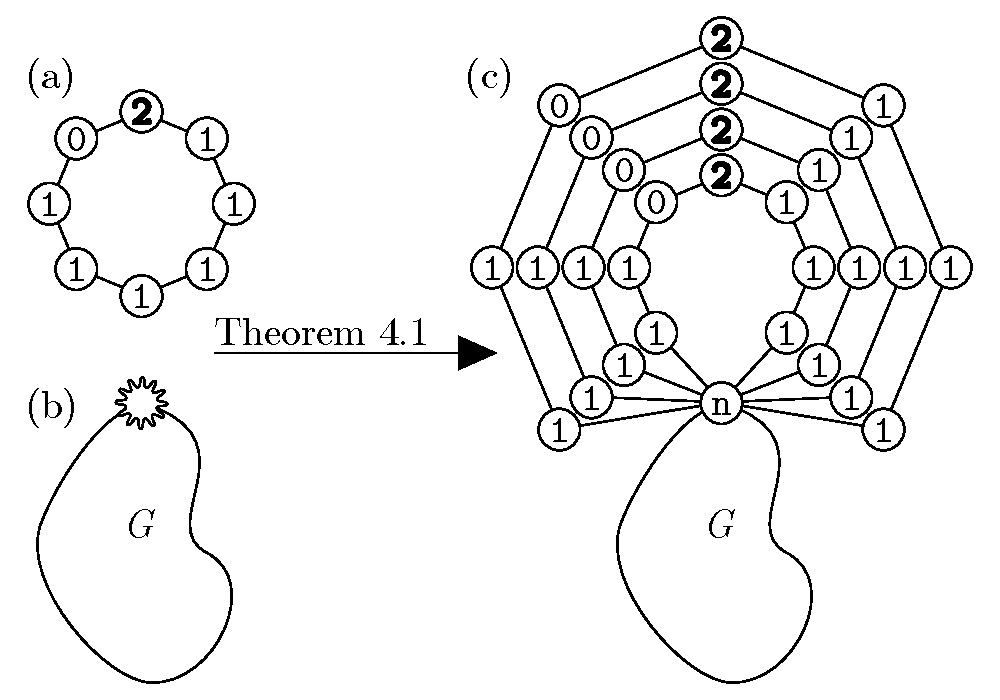
\includegraphics[width=\figWidthA]{Figures/natMotor}}
  \subfloat{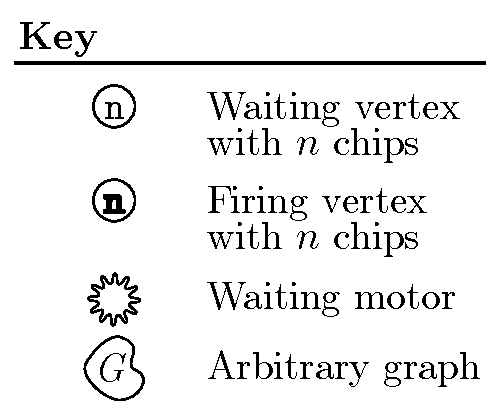
\includegraphics[width=\figWidthB]{Figures/keyShortish2}}
  \caption{Suppose the motor in motorized game (b) has firing sequence
    $(0,0,0,0,1,0,0,0,\dots)$. This occurs in ordinary game (a). By using
    sufficiently many copies of (a) and carefully choosing $n$, we construct
    (c). The behavior of $G$ in (c) is identical to the behavior of $G$ in
    (b).}
\label{natMot}
\end{figure}
\end{centering}

\begin{thm} \label{natMotors}
Let $\s$ be a periodic motorized game on $G$. If every motor's firing sequence
is possible, then there exists an ordinary game $\s'$ on a graph $H \supseteq
G$ such that
\begin{itemize}
\item $\firing[\s']{u}{t} = \firing{u}{t}$ for all $t \in \nats$ and $u \in
  \V$,
\item $\deg[H]{v} = \deg[G]{v}$ for all $v \in \V \setminus \mots$, and
\item the subgraph of $H$ induced by $V(G)$ is $G$. (That is, $H$ contains no
  edges between vertices of $G$ that are not also in $G$.)
\end{itemize}
\end{thm}

\begin{proof}
Our approach will be, for each $m \in \mots$, to attach many copies of a graph
with a vertex with $m$'s firing sequence to $m$. If sufficiently many copies
are attached, the number of chips $m$ has due to its neighbors in $G$ becomes
irrelevant as to whether or not it fires.

For each $m \in \mots$, let $A_m$ be a graph such that there exists a game
$\s^m$ and some vertex $u _m\in \V[A_m]$ such that $\firing[\s^m]{u_m}{t} =
\firing{m}{t}$ for all $t \in \nats$. Let $a_m$ and $b_m$ be the minimum and
maximum respectively of $\set{\chips{m}{t}}{t \in \nats}$. Let $k_m = b_m - a_m
+ 1$. Let $H$ be the union of $G$ and $k_m$ copies of each $A_m$, with $G$ and
the copies of $A_m$ disjoint except for $m = u_m$ for each $m \in
\mots$. (Thinking of the graphs as pointed topological spaces, each with
basepoint $m$ or $u_m$, $H$ is a wedge sum.)

It is clear by construction that $H$ contains no new edges between vertices of
$G$ and that
\begin{itemize}
\item $\deg[H]{m} = k_m\deg[{A_m}]{m} + \deg[G]{m}$ for all $m \in \mots$,
\item $\deg[H]{u} = \deg[{A_m}]{u}$ for all $u \in \V[A_m] \setminus \{m\}$ for
  each $m \in \mots$, and
\item $\deg[H]{v} = \deg[G]{v}$ for all $v \in \V \setminus \mots$.
\end{itemize}
Suppose that for some $t \in \nats$, $\pos[\s']{t}$ satisfies the following.
\begin{enumerate} \label{posAtT}
\item $\chips[\s']{m}{t} = k_m\chips[\s^m]{m}{t} + \deg[G]{m} + \chips{m}{t} -
  a_m$ for all $m \in \mots$.
\item $\chips[\s']{u}{t} = \chips[\s^m]{u}{t}$ for all $u \in \V[A_m] \setminus
  \{m\}$ for each $m \in \mots$.
\item $\chips[\s']{v}{t} = \chips{v}{t}$ for all $v \in \V \setminus \mots$.
\end{enumerate}
We will show that $\pos[\s']{t+1}$ satisfies the above as well. We have
$\deg[H]{v} = \deg[G]{v}$ for all $v \in \V \setminus \mots$, so
$\firing[\s']{v}{t} = \firing{v}{t}$ for all $v \in \V \setminus
\mots$. Similarly, $\firing[\s']{u}{t} = \firing[\s^m]{u}{t}$ for all $u \in
\V[A_m] \setminus \{m\}$ for each $m \in \mots$. Finally, for all $m \in
\mots$, if $\firing[\s^m]{m}{t} = 0$, then
\begin{align*}
  \chips[\s']{m}{t} &\leq k_m(\deg[{A_m}]{m)-1} + \deg[G]{m} + \chips{m}{t} -
  a_m \\
  &= k_m\deg[{A_m}]{m} + \deg[G]{m} + (\chips{m}{t} - b_m) - 1 \\
  &\leq \deg[H]{m} - 1,
\end{align*}
and if $\firing[\s^m]{m}{t} = 1$, then
\begin{align*}
  \chips[\s']{m}{t} &\geq k_m\deg[{A_m}]{m} + \deg[G]{m} + (\chips{m}{t} - a_m)
  \\
  &\geq \deg[H]{m},
\end{align*}
so $\firing[\s']{m}{t} = \firing[\s^m]{m}{t} = \firing{m}{t}$.

We know $\firing[\s']{v}{t} = \firing{v}{t}$ for all $v \in \V[H]$, so clearly
$\chips[\s']{v}{t+1} = \chips{v}{t+1}$ for all $v \in \V[G] \setminus \mots$
and $\chips[\s']{u}{t+1} = \chips[\s^m]{u}{t+1}$ for all $u \in \V[A_m]
\setminus \{m\}$ for each $m \in \mots$. Finally, we have
\begin{align*}
  \chips[\s']{m}{t+1} &= k_m\chips[\s^m]{m}{t} + \deg[G]{m} + \chips{m}{t} -
  a_m\ + \receiving[\s']{v}{t} - \firing[\s']{v}{t}\deg[H]{v} \\
  &= k_m\chips[\s^m]{m}{t} + \deg[G]{m} + \chips{m}{t} - a_m + \receiving{v}{t}
  - \firing{v}{t}\deg[G]{v}\ + \\
  &\qquad k_m\receiving[\s^m]{v}{t} - k_m\firing[\s^m]{v}{t}\deg[{A_m}]{v} \\
  &= k_m(\chips[\s^m]{m}{t} + \receiving[\s^m]{v}{t} -
  \firing[\s']{v}{t}\deg[{A_m}]{v)} + \deg[G]{m}\ + \\
  &\qquad (\chips{m}{t} + \receiving[\s]{v}{t} - \firing[\s]{v}{t}\deg[G]{v)} -
  a_m \\
  &= k_m\chips[\s^m]{m}{t+1} + \deg[G]{m} + \chips{m}{t+1} - a_m.
\end{align*}
for all $m \in \mots$.

We can distribute chips in $\pos[\s']{0}$ such that it satisfies (1), (2), and
(3), in which case, by induction, $\pos[\s']{t}$ satisfies (1), (2), and (3)
for all $t \in \nats$, implying $\firing[\s']{v}{t} = \firing{v}{t}$ for all $v
\in V(G)$.
\end{proof}

Again, we may relax the condition that the game be periodic. In this case, the
periodicity ensures that the number of chips on each motor is bounded. This is
easily shown to be equivalent to each motor having the same activity, so that
is a sufficient condition for the theorem. Of course, because all ordinary
games are eventually periodic, any motorized game in which each motor has a
possible firing sequence will eventually be periodic.

In Theorem~\ref{cheapLunch}, motors were primarily a convenient intuition and
terminology; we could have proved a similar theorem within the context of the
ordinary parallel chip-firing game, though its statement would have been
messier. Theorem~\ref{natMotors} demonstrates another way in which the motor
concept is useful, making certain conjectures easy to prove or disprove by
example.

\hidegame


\section{Signed Sums of Binary Sequences}\label{binSeq}
Throughout this section, if $b \in \{0,1\}$, we may write $\ol{b} = 1-b$.

We take a break from the parallel chip-firing game to consider two binary
strings $p$ and $q$ of length $n$. We denote the $i$\xth element of $p$ as
$p_i$. For simplicity, any integer equivalent to $i \bmod n$ may replace
$i$. Let a \emph{$b$-sector} of $p$, where $b \in \{0,1\}$, be an integer
interval $[x,y]$ such that
\begin{align*}
  p_x = p_{y-1} = p_y &= b \\
  p_{x-1} = p_{x-2} &= \ol{b} \\
  \forall i \in [x+1, y-3]: p_i + p_{i+1} &\neq 2\ol{b}.
\end{align*}
That is, the image of a 0-sector is preceded by two 1s, starts with 0, ends
with two 0s and contains no two consecutive 1s. The same statements with 0s and
1s swapped are true for 1-sectors.

It is easy to see that almost any string can be partitioned into 0- and
1-sectors in exactly one way, with exceptions only for always-alternating
strings (e.g.\ 010101) that can be thought of as one 0-sector or one
1-sector. Figure~\ref{sectorEx} has an example.

\begin{figure}
  \[
    \underbracket[1pt]{01000100}\overbracket[1pt]{11011}\underbracket[1pt]{00}
    \overbracket[1pt]{101011}
  \]
  \caption{A string's 0-sectors (marked below) and 1-sectors (marked
    above). Roughly speaking, $b$-sectors have no two $\ol{b}$s in a row and
    extend as far left as possible.}
  \label{sectorEx}
\end{figure}

Let
\begin{align*}
  s_i(p) &= \begin{cases}
    -1 & \text{if $i$ is in a 0-sector of $p$} \\
    1 & \text{if $i$ is in a 1-sector of $p$}
  \end{cases} \\
  \delta_i(p) &= \begin{cases}
    0 & \text{if $i$ is in a $b$-sector of $p$ and $i+1$ is in a $b$-sector of
      $p$} \\
    1 & \text{if $i$ is in a $b$-sector of $p$ and $i+1$ is in a
      $\ol{b}$-sector of $p$}.
  \end{cases}
\end{align*}
Our main theorem in this section concerns the sum
\begin{equation}\label{misbsum}
  M_S(p,q) = \sum_{i \in S}(s_i(p)(p_i - q_{i-1}) + s_i(q)(q_i - p_{i-1}) -
  \delta_i(p) - \delta_i(q)),
\end{equation}
where $S \subseteq [0, n-1]$. This sum, superficially speaking, measures each
sequence's ``disagreement'' with the other shifted back one step minus the
number of sector switches. The rules of the parallel chip-firing game put a
global upper bound on the total disagreement between vertices, yet the
following theorem says that sector switches require disagreement. We show in
Section~\ref{nonclumpiness} that this implies that firing sequences with sector
switches are impossible once a game has become periodic.

\begin{thm}\label{morale}
$M_{[0,n-1]}(p,q) \geq 0$.
\end{thm}

\begin{proof}
We can caculate $M_{[0,n-1]}(p,q)$ as $\sum_{i=0}^{n-1}M_{\{i\}}(p,q)$, and
$M_{\{i\}}(p,q)$ is determined by $p_{i-1}$, $p_i$, $s_i(p)$, $s_{i+1}(p)$, and
the same data for $q$. The motivation for using $s_{i+1}(p)$ as opposed to
$s_{i-1}(p)$ in $\delta_i(p)$ is that a switch away from a $b$-sector can occur
between $i$ and $i+1$ only if $p_{i-1} = p_i = b$. Let
\[
  \mu_i(p,q) = (p_{i-1},p_i,s_i(p),s_{i+1}(p),q_{i-1},q_i,s_i(q),s_{i+1}(q))
\]
and let $\G$ be a weighted digraph with
\begin{align*}
  \V[\G] &= \set{\mu_i(p,q)}{p,q \text{ strings}, i \in \nats} \\
  \E[\G] &= \set{(u,v,w)}{\exists p,q,i\colon
    u = \mu_i(p,q),
    v = \mu_{i+1}(p,q),
    w = M_{\{i\}}(p,q)}.
\end{align*}
(The third item of each edge is its weight.) Note that not every possible tuple
is a vertex. Define the weight of a path to be the sum of the weights of its
member edges, and call a path negative if it has negative weight. We can
calculate the $M_{[0,n-1]}(p,q)$ as the weight of a path induced by the
sequence of vertices $(\mu_0(p,q), \dots, \mu_{n-1}(p,q),
\mu_0(p,q))$. Therefore, it suffices to show that $\G$ has no negative
cycles. Running the Bellman-Ford algorithm~\cite{bellmanford} on $\G$ shows
this to be the case. We describe $\G$ and the algorithm in a Python program in
Figure~\ref{bfFig}.
\end{proof}

\begin{figure}[b!]
\SMALL
\verbatiminput{bellmanFord.py}
\normalsize
\caption{The Bellman-Ford algorithm run on $\G$.}
\label{bfFig}
\end{figure}
\FloatBarrier

\section{Nonclumpiness of Periodic Firing Patterns}\label{nonclumpiness}
We consider parallel chip-firing game $\s$ on undirected graph $G$. The
\emph{periodic firing pattern} (PFP) of a vertex $v \in \V$ is the binary
string
\[
  \firing{v}{t_0}\dots\firing{v}{t_0 + \period - 1},
\]
where $t_0$ is the smallest natural number such that $\pos{t_0}$ is
periodic. We write the PFP of $v$ as $\pfp{v}$. For simplicity, we assume here
that $t_0 = 0$ and index PFPs modulo $\period$.

Let $\pfps$ be the set of all PFPs occurring in $\s$. Call a PFP with both
consecutive 0s and consecutive 1s \emph{clumpy}, and let $\cpfps$ be the set of
all clumpy PFPs occurring in $\s$. (Recall that the $\period$\xth and 0\xth
entries of a PFP are the same, so, for example, 011010 is clumpy.) It is known
that, given any nonclumpy PFP, one can construct a parallel chip-firing game on
a simple cycle in which every vertex has that PFP shifted by some number of
steps~\cite{cycle}. We prove here that clumpy PFPs cannot occur in any parallel
chip-firing game, showing that a PFP is possible if and only if it is nonclumpy.

\begin{lem}\label{strongbg}
For all $v \in \V$ and $a, b \in \nats$,
\begin{equation}\label{local}
  -\deg{v} + 1 \leq \sum_{t=a}^{b}(\receiving{v}{t-1} - \deg{v}\firing{v}{t})
  \leq \deg{v}-1.
\end{equation}
\end{lem}

\begin{proof}
We express $\chips{v}{b}$ in terms of $\chips{v}{a-1}$.
\begin{align*}
  \chips{v}{b} &= \chips{v}{a-1} +
  \smashoperator{\sum_{t=a-1}}^{b-1}(\receiving{v}{t} - \deg{v}\firing{v}{t})
  \\
  \chips{v}{b} - \deg{v}\firing{v}{b} &= \chips{v}{a-1} -
  \deg{v}\firing{v}{a-1} + \sum_{t=a}^{b}(\receiving{v}{t-1} -
  \deg{v}\firing{v}{t})
\end{align*}
Recall that $0 \leq \chips{v}{t} - \deg{v}\firing{v}{t} \leq \deg{v} - 1$ for
all $t \in \nats$ such that $\pos{t}$ is periodic, which gives the desired
inequality.
\end{proof}

We define
\begin{align*}
\pfpverts{p} &= {\set{v \in \V}{\pfp{v}=p}} \\
\pfpedges{p}{q} &= {\set{\{v,w\} \in \E}{\pfp{v}=p, \pfp{w} = q}} \\
\misb{S}{p}{q} &= \sum_{i \in S}(p_{i} - q_{i-1})
\end{align*}
for binary strings $p$ and $q$. We now prove our main result: clumpy PFPs do
not occur in the parallel chip-firing game.

\begin{thm}\label{nct}
$\size{\pfpverts{p}} = 0$ for all $p \in \cpfps$.
\end{thm}

\begin{proof}
Roughly, summing an inequality given by Lemma~\ref{strongbg} over all vertices
with clumpy PFPs gives a lower bound on the same quantity, and summing an
inequality given by the Theorem~\ref{morale} over all edges incident with a
vertex with a clumpy PFP gives an upper bound on the same quantity. The lower
bound is the total number of vertices with clumpy PFPs, and the upper bound is
0.

Let $a,b \in \nats$ and $v \in \V$. Grouping the sum in \eqref{local} by $v$'s
neighbors instead of time steps yields
\[
  -\deg{v} + 1 \leq -\smashoperator{\sum_{w \in
      \N{v}}}\misb{[a,b]}{\pfp{v}}{\pfp{w}} \leq \deg{v} - 1.
\]
Regrouping gives us
\[
  1 \leq \smashoperator{\sum_{w \in \N{v}}}(1 +
  r\misb{[a,b]}{\pfp{v}}{\pfp{w}}),
\]
where $r = \pm1$. Let $p \in \pfps$. The above summed over $v \in \pfpverts{p}$
is
\[
  \size{\pfpverts{p}} \leq \smashoperator{\sum_{\substack{v \in \pfpverts{p}
        \\\ w \in \N{v}}}}(1 + r_v\misb{[a,b]}{p}{\pfp{w}}),
\]
where each $r_v = \pm1$ can depend on $v$. (Notation: ranges for outer sums are
above ranges for inner sums.)

For all $p \in \pfps$, let $\sctr{p}$ be the set of sectors of $p$. Abusing
notation slightly, we may write $s_X(p)$ instead of $s_i(p)$ if $i \in X \in
\sctr{p}$. Because each $X \in \sctr{p}$ is of the form $[a,b]$ for some $a,b
\in \nats$, we can sum the above inequality over $X \in \sctr{p}$ and $p \in
\cpfps$ to get
\begin{equation}\label{almost}
  \smashoperator[r]{\sum_{p \in \cpfps}}\size{\pfpverts{p}} \leq
  \smashoperator{\sum_{\substack{
        p \in \cpfps \\ v \in \pfpverts{p} \\
        w \in \N{v} \\ X \in \sctr{p}
  }}}(1 + r_{v,X}\misb{X}{p}{\pfp{w}}),
\end{equation}
where each $r_{v,X} = \pm1$ can depend on $v$ and $X$.

Let $p \in \cpfps$ and $q \in \pfps$. If $q$ is clumpy, then
\[
  M_{[0,\period-1]}(p,q) =
  \smashoperator{\sum_{X \in \sctr{p}}}(s_X(p)\misb{X}{p}{q} - 1) +
  \smashoperator{\sum_{X \in \sctr{q}}}(s_X(q)\misb{X}{q}{p} - 1).
\]
The $-1$ in each sum accounts for the $-\delta_i(p)-\delta_i(q)$ term in
\eqref{morale}, the definition of $M$. If instead $q$ is not clumpy, then
$\sctr{q} = \{[0,\period-1]\}$, so
\[
  M_{[0,\period-1]}(p,q) =
  \smashoperator{\sum_{X \in \sctr{p}}}(s_X(p)\misb{X}{p}{q} - 1) +
  s_{[0,\period-1]}(q)\misb{[0,\period-1]}{q}{p}.
\]
However, $\misb{[0,\period-1]}{q}{p} = 0$ because $p$ and $q$ have the same
length and number of 1s.

Let $W = \set{v \in \V}{\pfp{v} \in \cpfps}$ be the set of vertices with clumpy
PFPs. Choosing $r_{v,X} = -s_X(\pfp{v})$ and splitting the sum in
\eqref{almost} between neighbors with and without clumpy PFPs yields
\begin{align*}
  \smashoperator[r]{\sum_{\substack{
        p \in \cpfps \\
        X \in \sctr{p}
  }}}\size{\pfpverts{p}} &\leq
  \smashoperator{\sum_{\substack{
        p \in \cpfps \\ v \in \pfpverts{p} \\
        w \in \N{v} \cap W \\ X \in \sctr{p}
  }}}(1-s_X(p)\misb{X}{p}{\pfp{w}}) +
  \smashoperator{\sum_{\substack{
        p \in \cpfps \\ v \in \pfpverts{p} \\
        w \in \N{v} \setminus W \\ X \in \sctr{p}
  }}}(1-s_X(p)\misb{X}{p}{\pfp{w}}) \\
  &=
  \smashoperator[l]{\sum_{\substack{
        p,q \in \cpfps \\
        e \in \pfpedges{p}{q}
  }}}\!\!\Bigg(\smashoperator[r]{\sum_{X \in \sctr{p}}}(1-s_X(p)\misb{X}{p}{q})
  + \smashoperator{\sum_{X \in \sctr{q}}}(1-s_X(p)\misb{X}{q}{p})\Bigg)
  \\ &\qquad + 
  \smashoperator{\sum_{\substack{
        p \in \cpfps \\ v \in \pfpverts{p} \\
        w \in \N{v} \setminus W \\ X \in \sctr{p}
  }}}(1-s_X(p)\misb{X}{p}{\pfp{w}}) \\
  &= -\smashoperator{\sum_{\substack{
        p,q \in \cpfps \\
        e \in \pfpedges{p}{q}
  }}}M_{[0,\period-1]}(p,q) -
  \smashoperator{\sum_{\substack{
        p \in \cpfps \\
        v \in \pfpverts{p} \\ w \in \N{v} \setminus
        W}}}M_{[0,\period-1]}(p,F(w)) \\
  &\leq 0.
\end{align*}
The last line follows from Theorem~\ref{morale}, and when we sum over $p,q \in
\cpfps$, we consider $p$ and $q$ unordered. (A sum over $\{p,q\} \subseteq
\cpfps$ is one alternative notation.) Sets have nonnegative sizes, so
$\size{\pfpverts{p}} = 0$ for all $p \in \cpfps$.
\end{proof}


\section{Implications of Nonclumpiness} \label{corollaries}
It is a basic property of the parallel chip-firing game that every vertex fires
the same number of times each period~\cite{jiang}. This means, roughly
speaking, that every periodic game is either ``mostly waiting'' with bursts of
firing or ``mostly firing'' with bursts of waiting. (In fact, there is a
bijection between these two types of games. Each periodic game has a complement
that inverts firing and waiting~\cite{jiang}.) This is because if a vertex
waits twice in a row, then because it therefore never fires twice in a row, it
fires less than half the time over the course of a period. Similarly, a vertex
that fires twice in a row fires more than half the time. We cannot have a
vertex that waits twice in a row and a vertex that fires twice in a row in the
same periodic game because each vertex fires the same number of times each
period.

\begin{cor}
Once a parallel chip-firing game is periodic, either no vertex fires twice in a
row or no vertex waits twice in a row.
\end{cor}

That is, in periodic games, a firing sequence is possible if and only if it is
nonclumpy.

The \emph{interior} of a set of vertices $W$ is $\set{v \in W}{N(v) \subseteq
  W}$. Because a waiting (or firing) vertex with only waiting (or firing)
neighbors will wait (or fire) the following turn as well, the above observation
proves the following conjecture of Fey and Levine~\cite{privateComms}.

\begin{cor}\label{feyLevine}
Once a parallel chip-firing game is periodic, the interior of the set of
waiting vertices is always empty, the interior of set of firing vertices is
always empty, or both interiors are always empty.
\end{cor}

Interestingly, Corollary~\ref{feyLevine} also implies Theorem~\ref{nct}. If
clumpy PFPs were possible, then a leaf attached to a motor with a clumpy PFP
would be at different times in both the waiting and firing interiors.

In one of the first papers on the parallel chip-firing game, Bitar and Goles
characterized parallel chip-firing games on trees~\cite{bitarGoles}.
Corollary~\ref{freeLunch} and Theorem~\ref{nct} allow us to characterize the
behavior on tree-like subgraphs---subgraphs that, if an edge to a root vertex
is cut, become a tree separated from the rest of the graph---by making the root
vertex a motor.

\begin{cor}
Let $\s$ be a periodic game on $G$ with period at least 3 in which no vertex
fires twice in a row, $H$ be a tree-like subgraph of $G$, and $m \in \V[H]$ be
the root of $H$. Then for all $v \in \V[H]$,
\[
  \chips{v}{t} = \begin{cases}
    \deg{v} & \textnormal{if } \firing{m}{t-D} = 1 \\
    0 & \textnormal{if } \firing{m}{t-D-1} = 1 \\
    \deg{v} - 1 & \textnormal{otherwise},
  \end{cases}
\]
where $D$ is the distance from $m$ to $v$. An analogous result holds if no
vertex waits twice in a row.
\end{cor}

In some sense, tree-like subgraphs are passive in that their vertices fire only
in response to their root-side neighbor firing. In a periodic game, we can
completely remove tree-like subgraphs without affecting the PFPs of the other
vertices.

\begin{cor}
Let $\s$ be a periodic game on $G$, leaf $l \in \V$ have single neighbor $m$,
and $G'$ be $G$ with $l$ deleted. Then a game $\s'$ exists on $G'$ with the
same firing behavior as $\s$.
\end{cor}

The starting position $\pos[\s']{0}$ can agree with $\pos{0}$ completely except
for possibly removing a chip from $m$. We consider the case where no vertex
fires twice in a row. Compared to $\s'$, vertex $m$ has to have an extra chip
to fire in $\s$.  However, unless $m$ fired the previous turn---which, because
$l$ is a leaf, is equivalent to saying $l$ is firing this turn---$m$ will have
received the extra chip back from $l$, so removing both $l$ and the chip has no
effect on $m$ as long as $m$ does not fire while $l$ has a chip, which doesn't
happen due to nonclumpiness. The case where no vertex waits twice in a row is
analogous. This corollary concerns a leaf, though the result generalizes to all
tree-like subgraphs by repeated application, providing an alternate proof of
Corollary~\ref{freeLunch}.


\section{Discussion and Directions for Future Work} \label{discussion}

We have introduced motors, studied motorized games on trees, and shown that
motor-like behavior can be constructed in ordinary games, provided that each
motor has a possible firing sequence. We then showed that periodic firing
patterns are possible if and only if they are nonclumpy, which, among other
things, allows classification of periodic games as ``mostly waiting'' or
``mostly firing'' and the removal of tree-like subgraphs without loss of
generality.

We might expect that the space of motorized games be larger than that of
ordinary games. Theorem~\ref{natMotors} shows us that, as long as the firing
sequences involved are possible, the parallel chip-firing game is in some sense
just as ``expressive'' as its motorized variant. This allows, for example, the
simulation of some aspects of the \emph{dollar game}, a variant of the general
chip-firing game discussed by Biggs~\cite{biggs}. In the dollar game, exactly
one vertex, the ``government'', may have a negative number of chips and fires
if and only if no other vertices can fire. We can construct a motorized
parallel chip-firing game in which we replace the government with a motor that
waits a sufficiently large number of steps between each firing such that it
never fires in the same step as another vertex. Biggs showed that every dollar
game tends towards a critical position regardless of the order of vertex
firings, so this motorized parallel chip-firing game tends towards the same
critical position. Theorem~\ref{natMotors} may help reveal the extent to which
the parallel chip-firing game can simulate additional aspects of the dollar
game and other general chip-firing games.

% begin comment
\begin{comment}
\begin{centering}
  \begin{figure}[tbh]
    \subfloat{\includegraphics[width=\figWidthA]{Figures/motorizedTree}}
    \subfloat{\includegraphics[width=\figWidthB]{Figures/key}}
    \caption{A motor triggers a branching wave of gliders, one of which is
      shown.}
    \label{motorizedTree}
  \end{figure}
\end{centering}
\end{comment}
% end comment

Despite the expressiveness we get due to motors, the nonclumpiness of firing
patterns tells us that the parallel chip-firing game is ``easier'' than its
rules explicitly tell us it must be. In addition to results mentioned in
Section~\ref{corollaries}, Theorem~\ref{nct} is a step towards reducing the
parallel chip-firing game to one of interacting ``gliders''. For example,
consider the situation in Corollary~\ref{freeLunch}. Intuitively, we can think
of this corollary as stating that each firing of the motor creates a wave of
gliders that travels away from the motor. In fact, the corollary, together with
Theorem~\ref{nct}, implies that every periodic position on tree-like subgraphs
must be the result of such gliders, providing a new test that can diagnose some
positions that are never repeated. Every game on a simple cycle with period at
least 3 can be described by gliders~\cite{cycle}. (See Figure~\ref{cycleFig}.)
We believe that this approach could be used to analyze periodic behavior of
games on further classes of graphs, such as those in which each vertex is in at
most once cycle.

\begin{centering}
  \begin{figure}[tbh]
    \subfloat{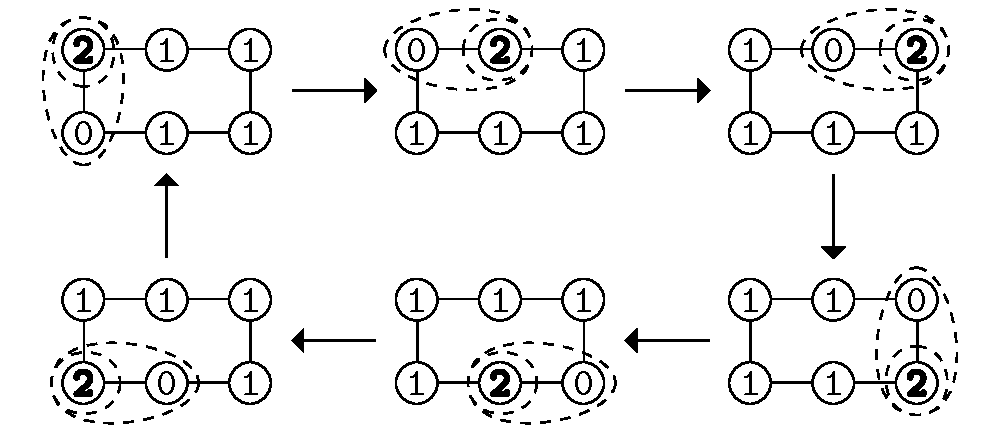
\includegraphics[width=\figWidthA]{Figures/cycle}}
    \subfloat{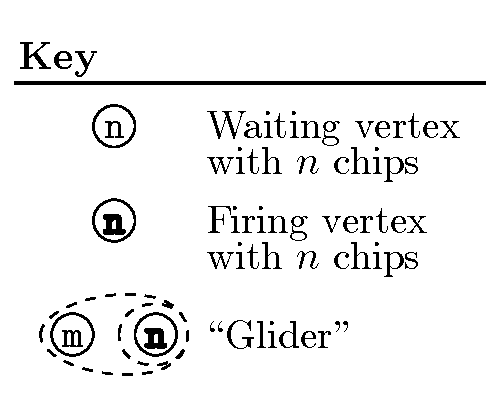
\includegraphics[width=\figWidthB]{Figures/keyShorter}}
    \caption{A game on a 6-cycle in which a glider orbits once each period.}
    \label{cycleFig}
  \end{figure}
\end{centering}

Nonclumpiness is essentially an unwritten rule of periods in the parallel
chip-firing game, which is unusual because no local property of the firing
mechanic disallows clumpiness. There are other graph automata, such as
\emph{source reversal}~\cite{sourceReversal} (essentially a parallel
chip-firing game with exactly one chip bound to each edge), that are more
restrictive than the parallel chip-firing game. For instance, nonclumpiness is
obvious for source reversal, even locally. In the other direction, motors make
it simple to show that certain stronger restrictions do not apply to the
parallel chip-firing game. For example, a path with the leaves are motors can
yield a game in which some chips cannot be bound to a single edge, which is is
a property of source reversal. We might ask which restrictions apply to which
chip-firing-style games. Is the parallel chip-firing game on undirected graphs
the most general game to which an analogue of Theorem~\ref{nct} applies?

We hope that the intuition and constructive powers of motors and the reduction
in the space of possible periodic games provided by nonclumpiness prove useful
in further research. \FloatBarrier


\appendix
\section{The Bellman-Ford Algorithm} \label{bfAlg}
The following Python program below constructs $\G$ from Section~\ref{binSeq}
and shows it has no negative cycles. For a more detailed exposition of the
Bellman-Ford algorithm and a proof of its validity, see~\cite{bellmanford}.

\bigskip
\SMALL
\verbatiminput{bellmanFord.py}
\normalsize


\section*{Acknowledgements}
We thank the MIT PRIMES program for supporting the research that brought us
together. We thank Tiankai Liu for improving upon a previous proof of
Theorem~\ref{morale}. We would also like to thank Anne Fey, Lionel Levine and
Tanya Khovanova for helpful discussions. Yan X Zhang was supported by an NSF
Graduate Fellowship.

\bibliographystyle{amsmodded}
\bibliography{refs}
\end{document}
